% Глава 1. Разведочный анализ датасета Glassdoor Job Reviews 2
%
% Длинные URL в списке источников: разрешаем более свободное
% выравнивание строк, чтобы ссылки не выходили за поле
\AtNextBibliography{\sloppy}
% Листинги кода не разрываются между страницами
\fvset{samepage=true}

\chapter{\MakeUppercase{Разведочный анализ данных с использованием PySpark}}\label{ch:first}
\section{Постановка задачи разведочного анализа}\vspace{\baselineskip}

Разведочный анализ данных (exploratory data analysis, EDA) --- этап исследования, на котором данные изучаются до построения моделей. На этом этапе определяются состав и качество данных, выявляются пропуски, ошибки и аномальные значения, оцениваются распределения признаков и взаимосвязи между ними~\cite{tukey1977eda}.

Исходными данными является датасет отзывов сотрудников о работодателях объёмом около 3,8~ГБ, содержащий почти 10~млн записей и размещённый в распределённой файловой системе HDFS кластера Apache Hadoop. При таком объёме обработка средствами одного компьютера неэффективна, поэтому вычисления выполняются фреймворком Apache Spark~\cite{karau2015spark, spark2022official}, задания которого распределяются по узлам кластера менеджером ресурсов YARN~\cite{white2013hadoop}. Требуется средствами DataFrame API библиотеки PySpark:
\begin{enumerate}
    \item определить типы признаков датасета;
    \item выявить пропущенные значения и устранить их;
    \item выявить выбросы и устранить их;
    \item рассчитать статистические показатели признаков (средние, среднеквадратичные отклонения, квартили и~т.\,д.);
    \item визуализировать распределения наиболее важных признаков;
    \item рассчитать корреляции между признаками.
\end{enumerate}

Кроме того, необходимо загрузить исходный файл, привести признаки к корректным типам и сохранить результаты обработки в таблицы формата Apache Iceberg.

Анализ выполнялся на кластере с использованием Apache Spark и Apache Iceberg. Драйвер работал в Jupyter-ноутбуке на узле кластера. Все операции над полными данными (фильтрация, группировка, агрегирование) выполнялись в Spark, а в библиотеку pandas передавались только агрегированные результаты небольшого объёма, необходимые для построения графиков~\cite{koirala2020pyspark, feng2021learning}.

\vspace{\baselineskip}\section{Описание датасета}\vspace{\baselineskip}

Для исследования выбран датасет Glassdoor Job Reviews~2~\cite{gauthier2024glassdoor}, размещённый на платформе Kaggle по адресу \url{https://www.kaggle.com/datasets/davidgauthier/glassdoor-job-reviews-2}. Он содержит отзывы сотрудников о компаниях-работодателях, опубликованные на сайте Glassdoor, где текущие и бывшие сотрудники анонимно оценивают условия работы. Датасет распространяется по лицензии CC~BY-NC-SA~4.0, допускающей учебное использование. В работе использована версия~3 от 15~октября 2024~года. Датасет состоит из файла \texttt{all\_reviews.csv} объёмом 3,8~ГБ с 19~столбцами и содержит 9\,901\,889~записей о 34\,374~компаниях за период с 25~января 2008~года по 26~июля 2023~года.

Каждая запись соответствует одному отзыву и включает общую оценку работодателя по шкале от~1 до~5, оценки по шести отдельным критериям (далее --- подоценки), мнение автора о компании, её генеральном директоре и перспективах, сведения об авторе и четыре текстовых поля. Мнения закодированы буквами: \texttt{v} --- положительное, \texttt{r} --- нейтральное, \texttt{x} --- отрицательное, \texttt{o} --- нет мнения. Используемые признаки перечислены в таблице~\ref{tab:features}. Исходные названия столбцов содержат пробелы и символы \texttt{/} и \texttt{\&}, неудобные в SQL-запросах, поэтому при загрузке столбцы были переименованы в стиле snake\_case.

\begin{table}[!ht]
    \centering
    \small
    \begin{tabularx}{\textwidth}{|p{4.6cm}|p{4.2cm}|X|}
        \hline
        \multicolumn{1}{|c|}{Столбец в файле} & \multicolumn{1}{c|}{Новое название} & \multicolumn{1}{c|}{Описание} \\ \hhline{|=|=|=|}
        rating                    & overall\_rating      & Общая оценка работодателя (1--5) \\ \hline
        title                     & headline             & Заголовок отзыва \\ \hline
        status                    & current              & Статус и стаж автора \\ \hline
        pros, cons                & pros, cons           & Тексты <<плюсы>> и <<минусы>> \\ \hline
        advice                    & advice               & Совет руководству \\ \hline
        Recommend                 & recommend            & Рекомендует ли автор компанию \\ \hline
        CEO Approval              & ceo\_approv          & Одобряет ли генерального директора \\ \hline
        Business Outlook          & outlook              & Оценка перспектив компании \\ \hline
        Career Opportunities      & career\_opp          & Карьерные возможности (1--5) \\ \hline
        Compensation and Benefits & comp\_benefits       & Зарплата и льготы (1--5) \\ \hline
        Senior Management         & senior\_mgmt         & Высшее руководство (1--5) \\ \hline
        Work/Life Balance         & work\_life\_balance  & Баланс работы и жизни (1--5) \\ \hline
        Culture \& Values         & culture\_values      & Культура и ценности (1--5) \\ \hline
        Diversity \& Inclusion    & diversity\_inclusion & Разнообразие и инклюзивность (1--5) \\ \hline
        firm\_link                & firm                 & Ссылка на страницу компании \\ \hline
        date                      & date\_review         & Дата публикации отзыва \\ \hline
        job                       & job\_title           & Должность автора \\ \hline
    \end{tabularx}
    \caption{Признаки датасета, используемые в работе}
    \label{tab:features}
\end{table}

При подготовке данных пустые строки заменены на \texttt{NULL}, а у значений удалены крайние пробелы. Из ссылки \texttt{firm\_link} регулярным выражением извлечено название компании (\texttt{Reviews/Calgary-Flames-Reviews-E5247.htm} $\to$ Calgary Flames). Даты вида <<Nov 19, 2022>> разобраны по шаблону \texttt{MMM d, yyyy}, оценки приведены к числовым типам, а коды мнений заменены категориями Positive, Mild, Negative и No opinion. Из строки статуса (<<Current Employee, more than 3 years>>) извлечены признаки \texttt{employee\_status} (Current или Former) и \texttt{tenure\_years} --- нижняя граница стажа в годах. Для текстовых полей вычислена длина в словах, после чего сами тексты, занимающие бо́льшую часть объёма, удалены. Результат сохранён в таблицу \texttt{glassdoor\_reviews} формата Apache Iceberg~\cite{iceberg2024docs} --- открытого табличного формата архитектуры LakeHouse~\cite{zaharia2021lakehouse}, хранящего данные в файлах Parquet вместе с метаданными таблицы.

\vspace{\baselineskip}\section{Определение типов признаков}\vspace{\baselineskip}

Во второй части работы таблица \texttt{glassdoor\_reviews} читается из каталога Iceberg и кэшируется в памяти исполнителей методом \texttt{cache}, поскольку используется многократно. Для каждого признака определены тип данных и приближённое число уникальных значений. Подсчёт выполнен функцией на алгоритме HyperLogLog++~\cite{heule2013hll}. В отличие от точного подсчёта, требующего перемешивания всех данных, она работает за один проход с погрешностью около 5~\%. Например, для признака \texttt{firm} получена оценка 33\,128 при точном значении 34\,374, то есть погрешность составила 3,6~\%. Типы признаков приведены в таблице~\ref{tab:types}.

\begin{table}[!ht]
    \centering
    \small
    \begin{tabularx}{\textwidth}{|>{\raggedright\arraybackslash}p{5.4cm}|X|>{\raggedright\arraybackslash}p{3.2cm}|}
        \hline
        \multicolumn{1}{|c|}{Признак} & \multicolumn{1}{c|}{Тип признака} & \multicolumn{1}{c|}{Уникальных (${\approx}$)} \\ \hhline{|=|=|=|}
        firm                         & категориальный номинальный             & 33\,128 \\ \hline
        job\_title                   & категориальный номинальный             & 458\,094 \\ \hline
        date\_review                 & дата                                   & 5\,447 \\ \hline
        employee\_status             & бинарный категориальный                & 2 \\ \hline
        recommend, ceo\_approv, outlook & категориальные порядковые           & 3; 4; 4 \\ \hline
        overall\_rating, подоценки   & порядковые (шкала 1--5)                & 5 \\ \hline
        tenure\_years                & количественный дискретный              & 6 \\ \hline
        headline\_words, pros\_words, cons\_words, advice\_words & количественные дискретные & 87; 778; 1\,399; 9 \\ \hline
    \end{tabularx}
    \caption{Типы признаков датасета}
    \label{tab:types}
\end{table}

Оценки по шкале 1--5 являются порядковыми признаками, однако при расчёте средних, квартилей и корреляций они, как принято в подобных исследованиях, рассматриваются как количественные дискретные. Мнения упорядочены как Negative~<~Mild~<~Positive и имеют дополнительную категорию No opinion. Столбец \texttt{current} полностью описывается производными признаками \texttt{employee\_status} и \texttt{tenure\_years}, поэтому удалён. В ходе анализа получены также количественный признак \texttt{year} (год отзыва) и порядковый признак \texttt{tenure\_group} (интервал стажа).

\vspace{\baselineskip}\section{Поиск и удаление дубликатов}\vspace{\baselineskip}

Уникального ключа отзыва в датасете нет, поэтому дубликатами считались строки, совпадающие по всем признакам. Группировка по всем столбцам выявила 609\,412 групп повторяющихся строк, например, набор отзывов об одной компании повторён в файле 2\,426 раз. Дубликаты удалены методом \texttt{dropDuplicates}, а именно удалено 846\,660~строк (8,55~\%), осталось 9\,055\,229. Поиск одинаковых строк требует перемешивания данных, поэтому результат был закэширован, а прежний кэш освобождён методом \texttt{unpersist}. Ограничение метода состоит в том, что вместо самих текстов сравнивалась их длина в словах, поэтому изредка два похожих коротких отзыва могли быть приняты за один. При группах из тысяч одинаковых строк это не меняет вывода: большая часть удалённых строк --- настоящие дубликаты.

\vspace{\baselineskip}\section{Определение и устранение пропущенных значений}\vspace{\baselineskip}

Для подсчёта пропусков создана функция \texttt{null\_report}, передающая в один вызов \texttt{agg} агрегаты для всех столбцов. Все агрегаты входят в один запрос, поэтому Spark подсчитывает пропуски во всех столбцах одним заданием, за один проход по данным. Результат показан на рисунке~\ref{fig:missing}.

\begin{figure}[!ht]
    \centering
    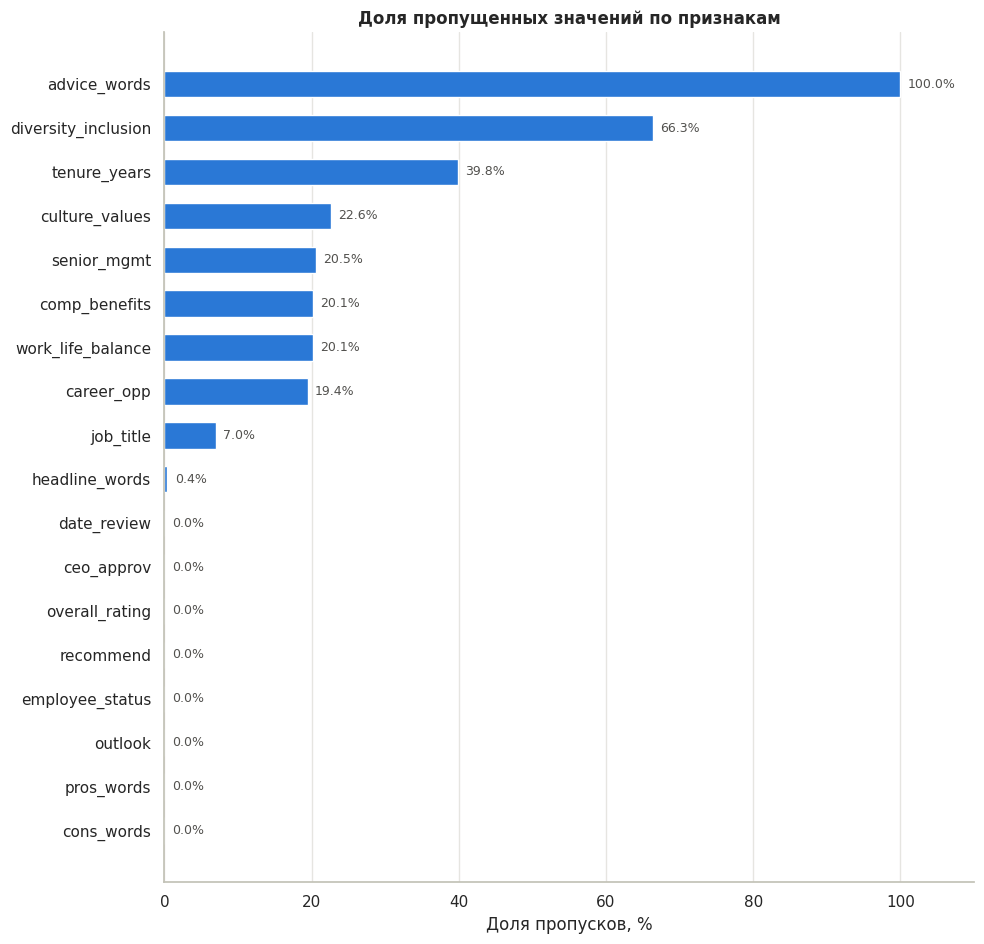
\includegraphics[width=0.62\textwidth]{Content/Images/glassdoor_missing.png}
    \caption{Доля пропущенных значений по признакам}
    \label{fig:missing}
\end{figure}

Пропуски распределены неравномерно, и их причины различны. Совет руководству (\texttt{advice\_words}) заполнен лишь в 13~отзывах, то есть в этой версии датасета поле фактически не собрано. Подоценка \texttt{diversity\_inclusion} отсутствует в 66,3~\% отзывов, так как Glassdoor ввёл её лишь осенью 2020~года~\cite{maurer2020dei}, поэтому у более ранних отзывов её, как правило, нет. Это пример неслучайных пропусков. Стаж не указан в 39,8~\% отзывов, остальные подоценки пропущены в 19,4--22,6~\%, должность --- в 7~\%. Кроме того, в 145~строках одновременно отсутствуют дата, общая оценка и все мнения --- это повреждённые записи.

Пропуски обрабатывались по следующим правилам:
\begin{enumerate}
    \item строки без ключевых признаков (компания, дата, общая оценка) удаляются;
    \item в категориальных признаках пропуски заменяются категорией Unknown;
    \item количественный признак с долей пропусков более 50~\% удаляется, поскольку заполнение большей части значений исказило бы его распределение;
    \item в остальных количественных признаках пропуски заменяются медианой, которая, в отличие от среднего, устойчива к перекосам распределения и всегда является допустимым значением шкалы;
    \item пропуск в длине текста означает, что текст не написан, и заменяется нулём.
\end{enumerate}

Медиана вычисляется методом \texttt{approxQuantile}, реализующим вариант алгоритма Гринвальда--Ханны~\cite{greenwald2001quantiles}, который находит квантиль с заданной погрешностью без полной сортировки данных. В результате удалены 145~повреждённых строк, после чего пропуски в общей оценке и мнениях исчезли, а в датасете осталось 9\,055\,084~строки. Подоценка \texttt{diversity\_inclusion} удалена. Пропуски в подоценках \texttt{work\_life\_balance} и \texttt{culture\_values} заполнены медианой~4, в \texttt{career\_opp}, \texttt{comp\_benefits} и \texttt{senior\_mgmt} --- медианой~3. Влияние заполнения на распределения показано на рисунке~\ref{fig:imputation}.

\begin{figure}[!ht]
    \centering
    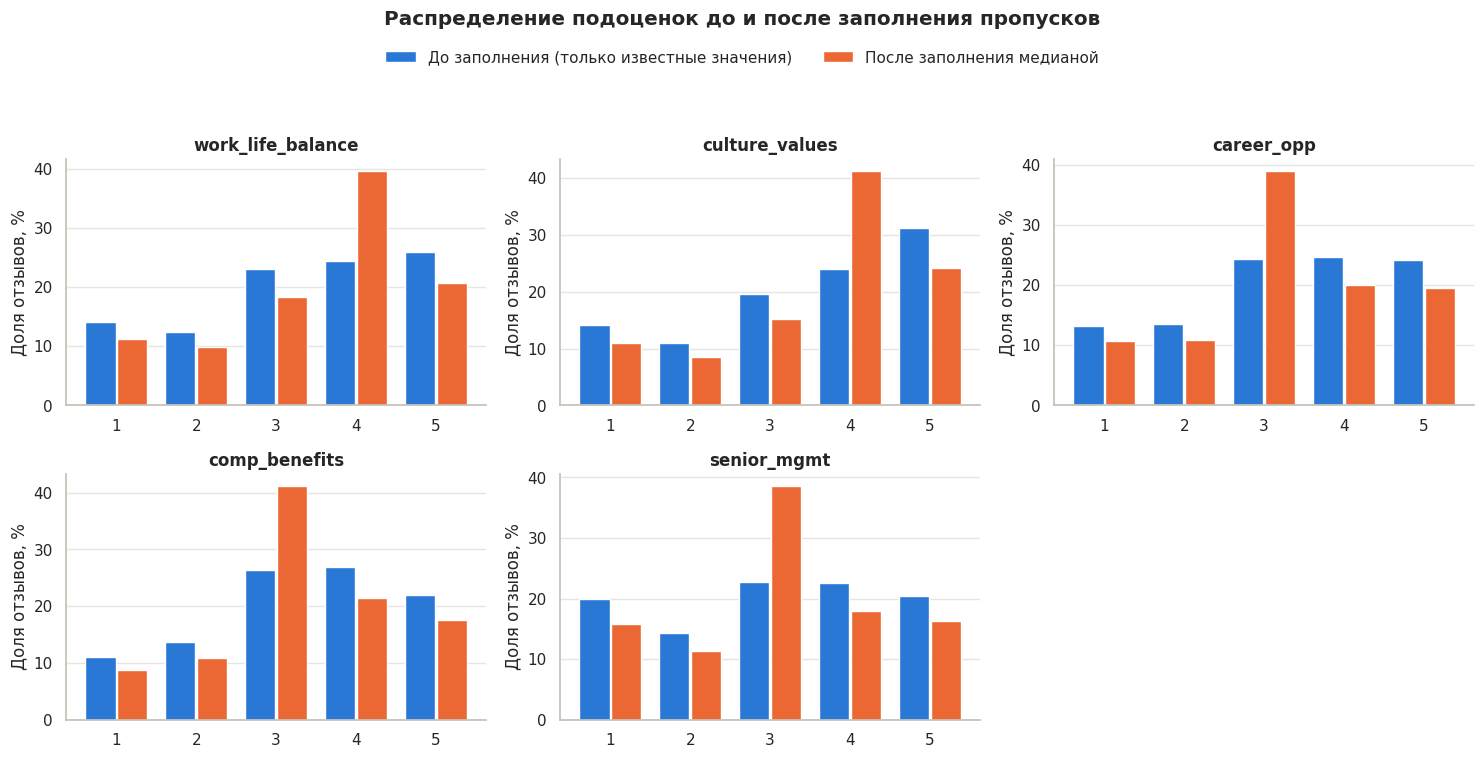
\includegraphics[width=0.9\textwidth]{Content/Images/glassdoor_imputation.png}
    \caption{Распределения подоценок до и после заполнения пропусков медианой}
    \label{fig:imputation}
\end{figure}

Заполнение увеличивает долю медианного значения до 38--41~\% и уменьшает разброс признаков --- известный недостаток заполнения константой. Заполнение подоценки общей оценкой того же отзыва дало бы более правдоподобные значения, но искусственно усилило бы их взаимосвязь, поэтому выбран более нейтральный вариант. Пропуски в \texttt{tenure\_years} заполнены медианой, равной одному году. Чтобы сохранить сведения о неуказанном стаже, предварительно создан признак \texttt{tenure\_group} с отдельной категорией Unknown. Должность скрыта значением Anonymous Employee в 1\,567\,716~отзывах; по сути это тоже пропуск, поэтому такие значения вместе с пустыми (всего 24,26~\%) заменены на Unknown. После замены пропусков нулями признак \texttt{advice\_words} стал константой, неинформативной для анализа. Итоговая проверка показала, что пропусков в данных не осталось.

\vspace{\baselineskip}\section{Выявление и устранение выбросов}\vspace{\baselineskip}

Для поиска выбросов использован метод межквартильного размаха (IQR), лежащий в основе диаграммы <<ящик с усами>>~\cite{tukey1977eda}. Выбросом считается значение, выходящее за границы
\begin{equation}
    \label{eq:iqr}
    L = Q_1 - 1{,}5 \cdot IQR, \quad U = Q_3 + 1{,}5 \cdot IQR, \quad IQR = Q_3 - Q_1,
\end{equation}
где $Q_1$ и $Q_3$ --- первый и третий квартили.

\textbf{Оценки.} Все значения оценок лежат в пределах шкалы 1--5. Для общей оценки $Q_1 = 3$, $Q_3 = 5$, и по формуле~(\ref{eq:iqr}) границы равны 0 и 8, так что выбросов нет. Результаты для подоценок приведены в таблице~\ref{tab:subratings} и на рисунке~\ref{fig:subratings}.

\begin{table}[!ht]
    \centering
    \small
    \begin{tabularx}{\textwidth}{|X|c|c|c|c|c|c|}
        \hline
        \multicolumn{1}{|c|}{Подоценка} & $Q_1$ & Медиана & $Q_3$ & $L$ & $U$ & Выбросов, \% \\ \hhline{|=|=|=|=|=|=|=|}
        work\_life\_balance & 3 & 4 & 4 & 1,5  & 5,5 & 11,26 \\ \hline
        culture\_values     & 3 & 4 & 4 & 1,5  & 5,5 & 10,91 \\ \hline
        career\_opp         & 3 & 3 & 4 & 1,5  & 5,5 & 10,64 \\ \hline
        comp\_benefits      & 3 & 3 & 4 & 1,5  & 5,5 & 8,78 \\ \hline
        senior\_mgmt        & 2 & 3 & 4 & $-1$ & 7   & 0,00 \\ \hline
    \end{tabularx}
    \caption{Границы выбросов подоценок по методу IQR}
    \label{tab:subratings}
\end{table}

\begin{figure}[!ht]
    \centering
    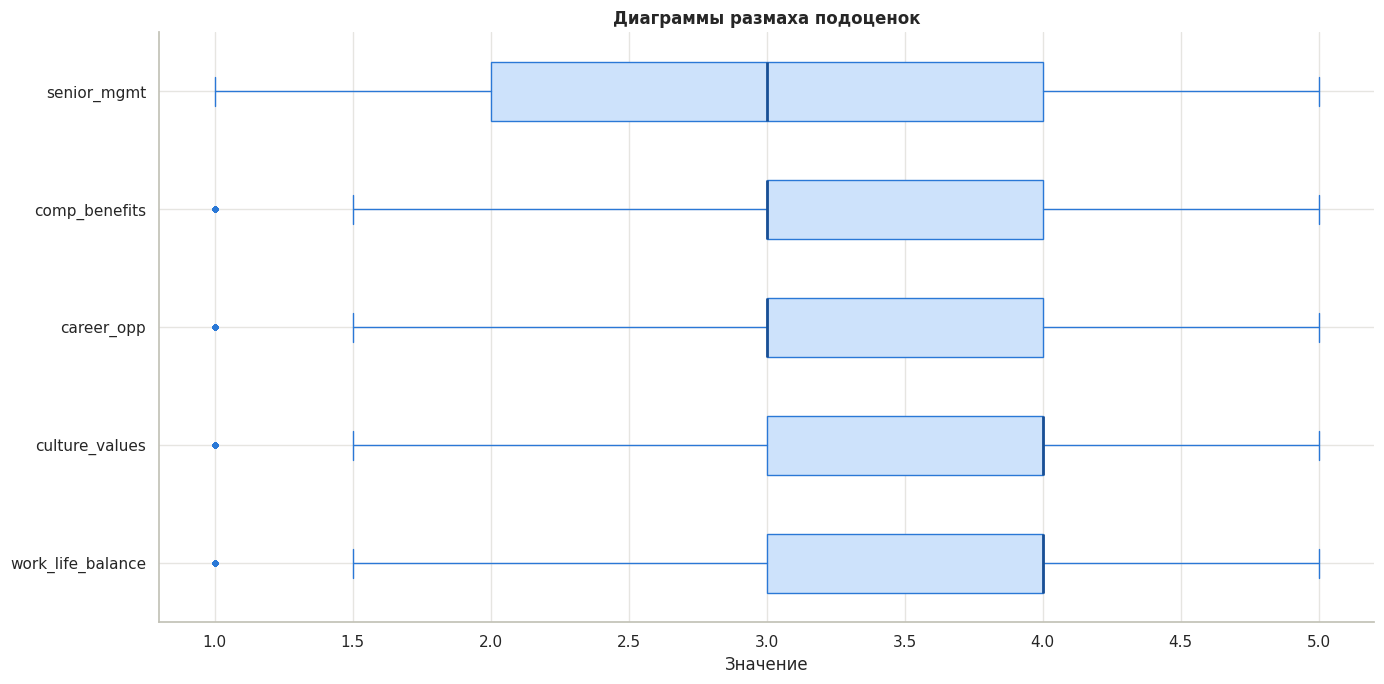
\includegraphics[width=0.85\textwidth]{Content/Images/glassdoor_subratings_box.png}
    \caption{Диаграммы размаха подоценок после заполнения пропусков}
    \label{fig:subratings}
\end{figure}

У четырёх подоценок межквартильный размах равен единице, и к выбросам формально относятся все оценки~1 --- около миллиона строк для каждой подоценки. Отчасти это следствие заполнения медианой, сблизившего квартили. Однако оценка~1 --- допустимое значение шкалы, выражающее крайнее недовольство, а не ошибка, поэтому такие строки не удалялись. Этот пример показывает, что правило IQR нельзя механически применять к порядковым шкалам с малым числом значений.

\textbf{Число отзывов на компанию.} На одну компанию в среднем приходится 263,4~отзыва при среднеквадратичном отклонении 1\,947,9, однако медиана равна 8, а квартили --- 2 и 53. Максимум, 134\,603~отзыва, принадлежит компании Amazon (рисунок~\ref{fig:firms}). По формуле~(\ref{eq:iqr}) выбросами являются все компании, у которых больше 130~отзывов. Однако это не ошибки, а крупные работодатели, поэтому их отзывы сохранены. Следует лишь учитывать, что агрегированные показатели во многом отражают мнение сотрудников крупных компаний. Неравномерность ключа влияет и на производительность Spark: при группировке по \texttt{firm} все строки крупной компании попадают в один раздел, и обрабатывающая его задача выполняется дольше остальных (перекос данных, data skew).

\begin{figure}[!ht]
    \centering
    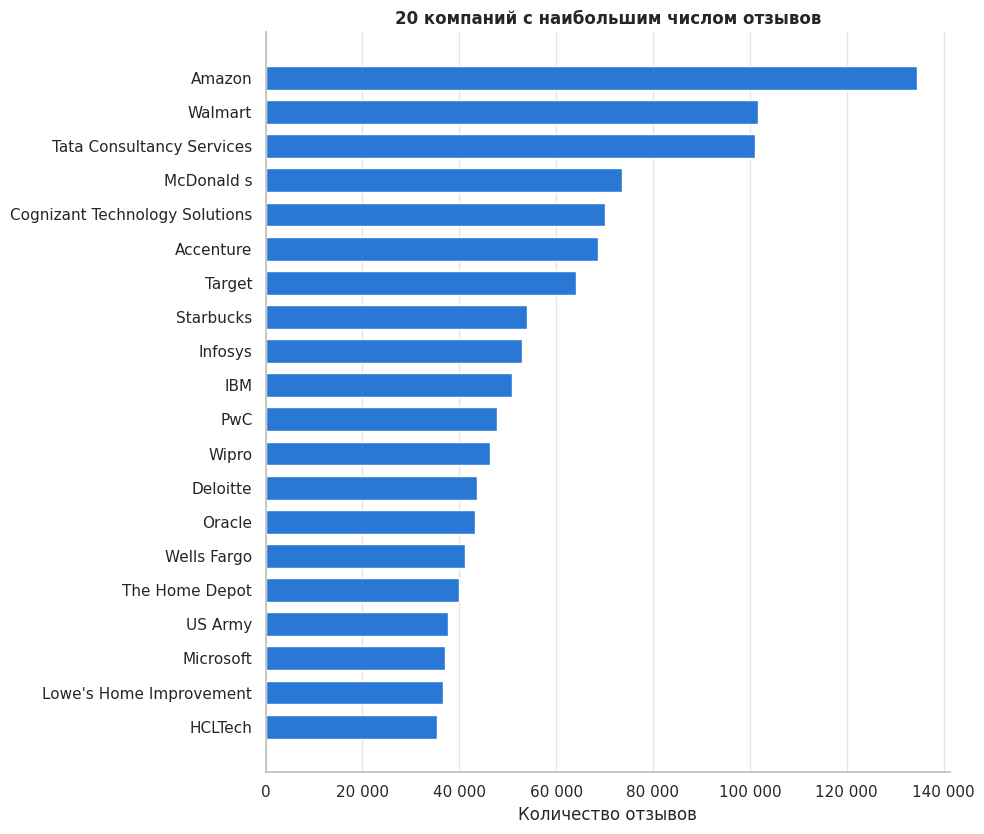
\includegraphics[width=0.58\textwidth]{Content/Images/glassdoor_top_firms.png}
    \caption{Двадцать компаний с наибольшим числом отзывов}
    \label{fig:firms}
\end{figure}

\textbf{Длина текстов.} Распределения длин текстов имеют длинный правый хвост (рисунок~\ref{fig:words}). Медиана длины <<плюсов>> составляет 8~слов при максимуме 3\,153, <<минусов>> --- 9 при максимуме 7\,019, заголовка --- 3 при максимуме 328. По правилу IQR выбросами являются 5,50~\% заголовков, 10,11~\% <<плюсов>> и 10,95~\% <<минусов>>, то есть каждый десятый обычный отзыв, поэтому для распределения с длинным хвостом это правило слишком строгое.

\begin{figure}[!ht]
    \centering
    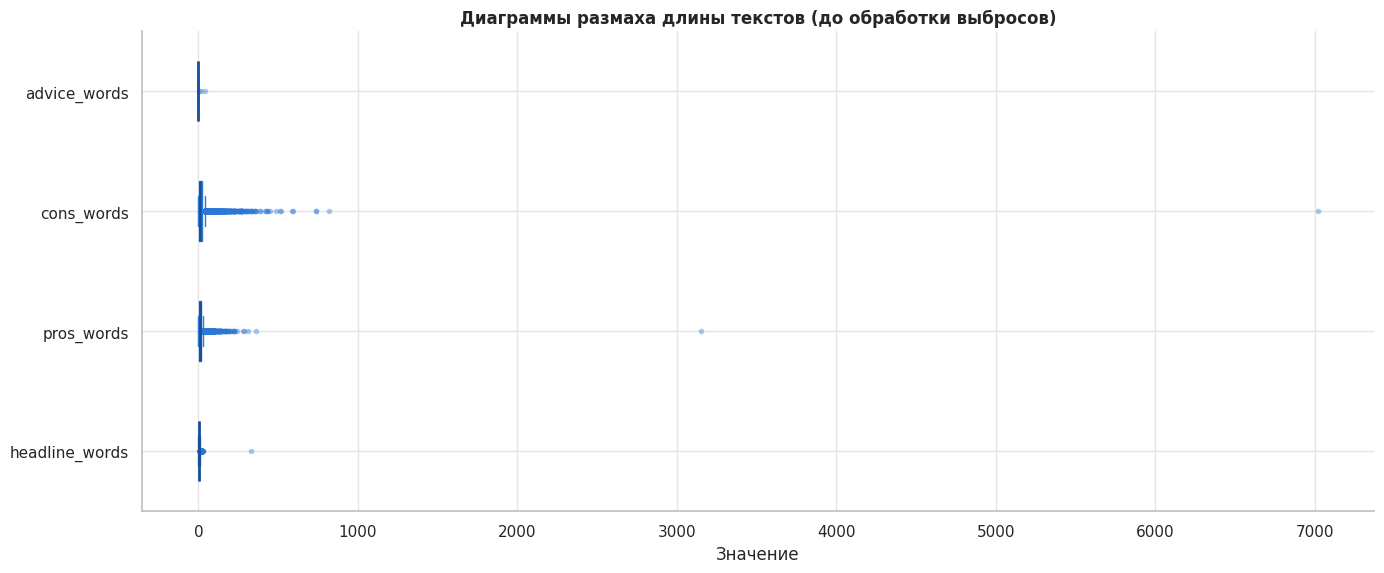
\includegraphics[width=0.85\textwidth]{Content/Images/glassdoor_words_box.png}
    \caption{Диаграммы размаха длины текстов до обработки выбросов}
    \label{fig:words}
\end{figure}

Вместо удаления строк применена винзоризация: значения выше 99-го перцентиля заменены самим перцентилем. Границы составили 16~слов для заголовка, 87 --- для <<плюсов>> и 182 --- для <<минусов>>; изменено около 1~\% значений каждого признака (от 79 до 99~тыс.). Строки не удалялись, а среднеквадратичное отклонение длины <<минусов>> снизилось с 41,6 до 28,8~слова. Распределение длины <<плюсов>> после обработки показано на рисунке~\ref{fig:pros}.

\begin{figure}[!ht]
    \centering
    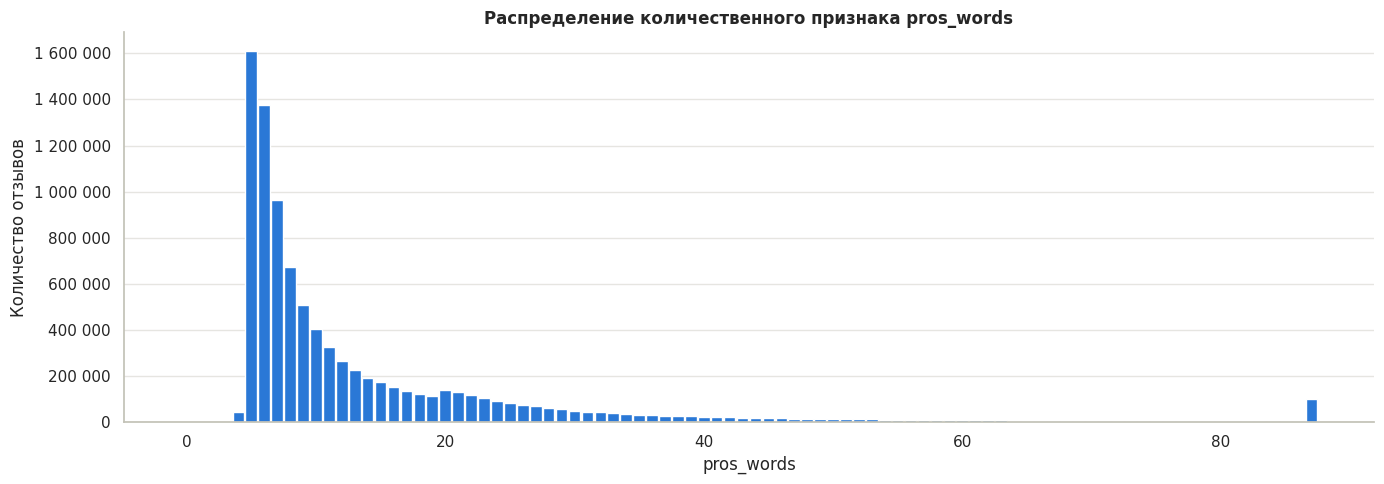
\includegraphics[width=0.85\textwidth]{Content/Images/glassdoor_pros_hist.png}
    \caption{Распределение длины текста <<плюсы>> после ограничения 99-м перцентилем}
    \label{fig:pros}
\end{figure}

Тексты короче пяти слов практически отсутствуют, а самое частое значение равно ровно пяти словам. Вероятно, форма отзыва на сайте требует минимальной длины этого поля. Столбец у правой границы гистограммы образуют значения, ограниченные 99-м перцентилем.

\vspace{\baselineskip}\section{Статистические показатели признаков}\vspace{\baselineskip}

В данной работе были рассчитаны статистические показатели количественных признаков за один проход по данным. Результаты приведены в таблице~\ref{tab:stats}.

\begin{table}[!ht]
    \centering
    \small
    \begin{tabularx}{\textwidth}{|X|c|c|c|c|c|c|c|}
        \hline
        \multicolumn{1}{|c|}{Признак} & Среднее & СКО & Мин. & $Q_1$ & Медиана & $Q_3$ & Макс. \\ \hhline{|=|=|=|=|=|=|=|=|}
        overall\_rating     & 3,55    & 1,25  & 1    & 3    & 4    & 5    & 5 \\ \hline
        work\_life\_balance & 3,49    & 1,24  & 1    & 3    & 4    & 4    & 5 \\ \hline
        culture\_values     & 3,59    & 1,24  & 1    & 3    & 4    & 4    & 5 \\ \hline
        career\_opp         & 3,27    & 1,20  & 1    & 3    & 3    & 4    & 5 \\ \hline
        comp\_benefits      & 3,28    & 1,14  & 1    & 3    & 3    & 4    & 5 \\ \hline
        senior\_mgmt        & 3,07    & 1,25  & 1    & 2    & 3    & 4    & 5 \\ \hline
        tenure\_years       & 2,10    & 2,49  & 0    & 1    & 1    & 3    & 10 \\ \hline
        headline\_words     & 3,76    & 2,95  & 0    & 2    & 3    & 5    & 16 \\ \hline
        pros\_words         & 13,91   & 14,24 & 0    & 6    & 8    & 16   & 87 \\ \hline
        cons\_words         & 20,26   & 28,79 & 0    & 6    & 9    & 21   & 182 \\ \hline
        year                & 2018,76 & 3,24  & 2008 & 2016 & 2020 & 2021 & 2023 \\ \hline
    \end{tabularx}
    \caption{Статистические показатели количественных признаков}
    \label{tab:stats}
\end{table}

Средняя общая оценка составляет 3,55 при медиане~4, то есть распределение смещено к высоким оценкам. Выше всех подоценок оценена корпоративная культура (3,59), за ней следуют баланс работы и жизни (3,49), зарплата и льготы (3,28) и карьерные возможности (3,27). Ниже всех оценено высшее руководство (3,07); у этой подоценки и наибольший разброс: четверть авторов ставит руководству 1 или~2. Средние подоценок рассчитаны после заполнения пропусков и несколько смещены к медиане. <<Минусы>> в среднем длиннее <<плюсов>> (20,3 слова против 13,9): о недостатках работодателя авторы пишут подробнее. Половина отзывов опубликована в 2020~году или позже.

Для категориальных признаков рассчитаны число категорий, мода и её доля в таблице~\ref{tab:catstats}. Признаки \texttt{firm} и \texttt{job\_title} имеют очень высокую кардинальность, а именно даже самая частая конкретная должность, Sales Associate, встречается лишь в 1,62~\% отзывов. Мнения о генеральном директоре и перспективах компании отсутствуют более чем у трети авторов.

\begin{table}[!ht]
    \centering
    \small
    \begin{tabularx}{\textwidth}{|X|c|c|c|}
        \hline
        \multicolumn{1}{|c|}{Признак} & Категорий (${\approx}$) & Мода & Доля моды, \% \\ \hhline{|=|=|=|=|}
        firm             & 33\,128  & Amazon     & 1,49 \\ \hline
        job\_title       & 458\,094 & Unknown    & 24,26 \\ \hline
        employee\_status & 3        & Current    & 57,59 \\ \hline
        recommend        & 3        & Positive   & 46,45 \\ \hline
        ceo\_approv      & 4        & No opinion & 38,06 \\ \hline
        outlook          & 4        & No opinion & 35,55 \\ \hline
        tenure\_group    & 7        & Unknown    & 39,84 \\ \hline
    \end{tabularx}
    \caption{Показатели категориальных признаков}
    \label{tab:catstats}
\end{table}

\vspace{\baselineskip}\section{Визуализация распределений наиболее важных признаков}\vspace{\baselineskip}

Для построения графиков подсчёт выполняется в Spark операциями \texttt{groupBy} и \texttt{agg}, а в pandas передаётся только результат из нескольких десятков строк. Для гистограмм номер интервала каждого значения также вычисляется в Spark.

\textbf{Общая оценка.} Распределение целевого признака \texttt{overall\_rating} показано на рисунке~\ref{fig:rating}. Чаще всего выставляется оценка~4 (29,79~\%), затем~5 (27,07~\%) и~3 (23,22~\%); оценки 1 и 2 встречаются в 9,49 и 10,43~\% отзывов. Таким образом, высокие оценки ставят 56,9~\% авторов, а низкие --- 19,9~\%.

\begin{figure}[!ht]
    \centering
    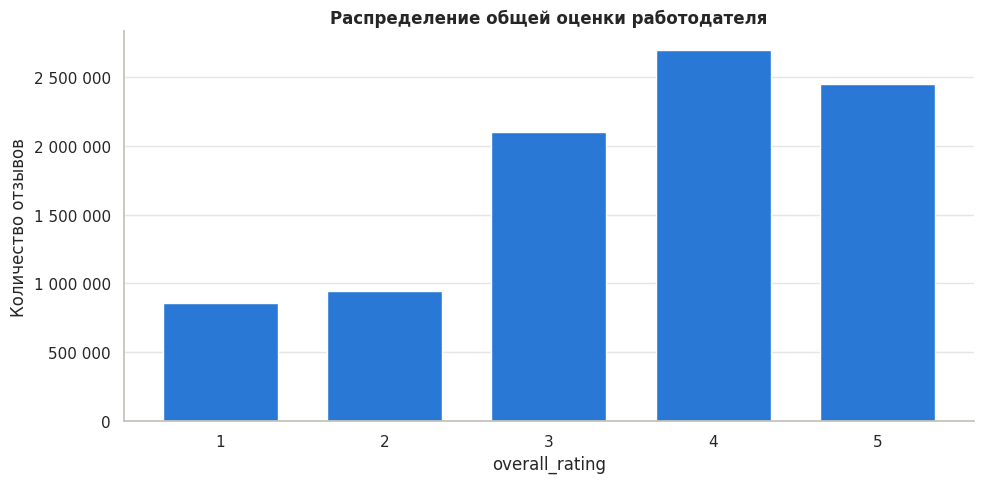
\includegraphics[width=0.65\textwidth]{Content/Images/glassdoor_rating_dist.png}
    \caption{Распределение общей оценки работодателя}
    \label{fig:rating}
\end{figure}

\textbf{Динамика по годам} показана на рисунке~\ref{fig:years}. Число отзывов выросло с 34\,983 в 2008~году до 1\,799\,845 в 2021~году; на 2021--2022~годы приходится 37,9~\% датасета, а данные за 2023~год неполные. Средняя оценка выросла с 3,05 в 2010~году до 3,72 в 2022~году, особенно резко --- между 2019 и 2020~годами (с 3,52 до 3,69). Причины роста по имеющимся данным установить нельзя. Возможными объяснениями являются изменения правил сбора отзывов, привлечение работодателями сотрудников к написанию отзывов и изменение состава компаний в выборке. Поэтому оценки разных лет непосредственно не сопоставимы.

\begin{figure}[!ht]
    \centering
    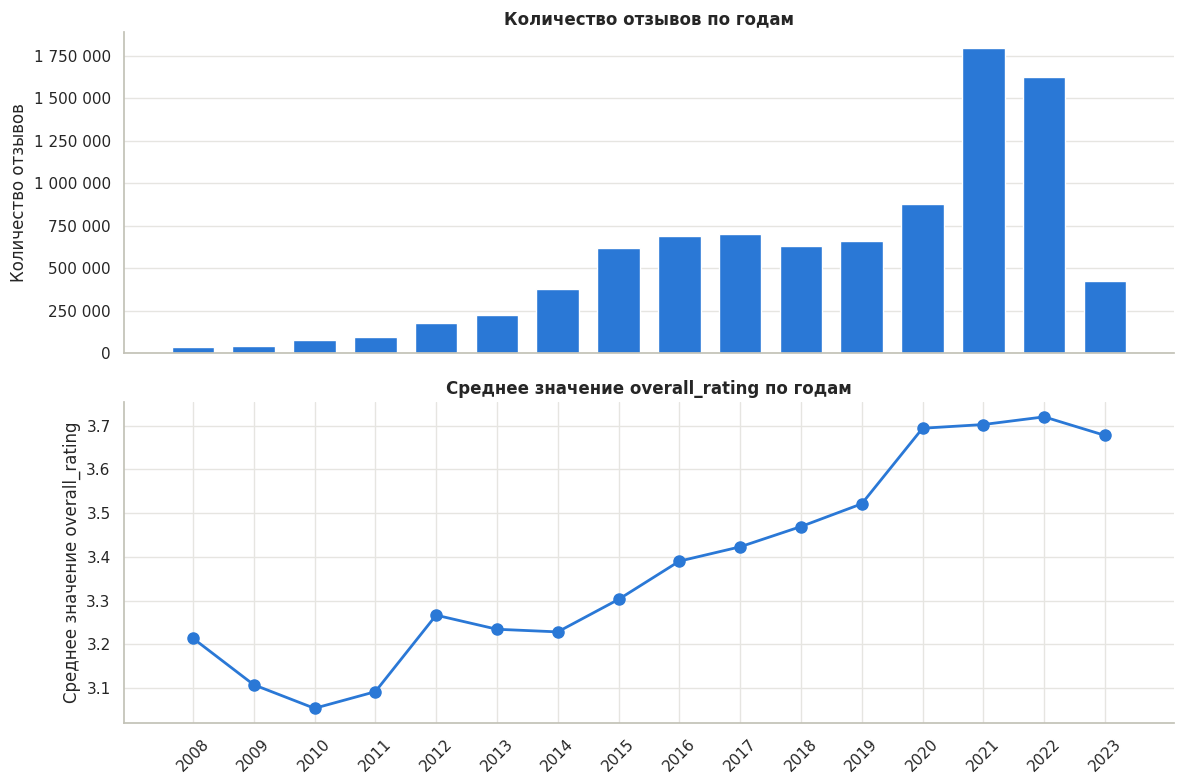
\includegraphics[width=0.8\textwidth]{Content/Images/glassdoor_by_year.png}
    \caption{Количество отзывов и средняя общая оценка по годам}
    \label{fig:years}
\end{figure}

\textbf{Мнения о компании.} Распределения мнений и средняя общая оценка в каждой категории приведены в таблице~\ref{tab:opinions}. Для рекомендации компании категория Mild отсутствует: на этот вопрос можно ответить только <<да>> или <<нет>>.

\begin{table}[!ht]
    \centering
    \small
    \begin{tabularx}{\textwidth}{|X|c|c|c|c|c|c|}
        \hline
        \multirow{2}{*}{Мнение} & \multicolumn{2}{c|}{recommend} & \multicolumn{2}{c|}{ceo\_approv} & \multicolumn{2}{c|}{outlook} \\ \cline{2-7}
         & Доля, \% & Оценка & Доля, \% & Оценка & Доля, \% & Оценка \\ \hhline{|=|=|=|=|=|=|=|}
        Positive   & 46,45 & 4,22 & 32,46 & 4,17 & 34,30 & 4,23 \\ \hline
        Mild       & ---   & ---  & 19,22 & 3,12 & 16,80 & 3,15 \\ \hline
        Negative   & 24,73 & 2,14 & 10,26 & 2,04 & 13,35 & 2,08 \\ \hline
        No opinion & 28,82 & 3,67 & 38,06 & 3,64 & 35,55 & 3,62 \\ \hline
    \end{tabularx}
    \caption{Распределение мнений и средняя общая оценка по категориям}
    \label{tab:opinions}
\end{table}

По всем трём признакам средняя оценка монотонно растёт от отрицательного мнения к положительному. Сильнее всего различаются группы по рекомендации: 4,22 у рекомендующих компанию против 2,14 у не рекомендующих, то есть разница составляет 2,08~балла. Авторы без мнения оценивают компанию на 3,6--3,7, близко к средней по датасету.

\textbf{Статус и стаж автора.} Текущие сотрудники (57,59~\%) оценивают работодателя в среднем на 3,75, бывшие (42,41~\%) --- на 3,27. Разница почти в полбалла ожидаема, поскольку недовольные условиями работы чаще увольняются. Зависимость оценки от стажа приведена в таблице~\ref{tab:tenure}. На сайте стаж задаётся интервалами, поэтому, например, категория <<более 1 года>> означает стаж от 1 до 3~лет.

\begin{table}[!ht]
    \centering
    \small
    \begin{tabularx}{\textwidth}{|X|c|c|c|}
        \hline
        \multicolumn{1}{|c|}{Стаж} & Отзывов & Доля, \% & Средняя оценка \\ \hhline{|=|=|=|=|}
        менее 1 года  & 1\,190\,066 & 13,14 & 3,510 \\ \hline
        1--3 года     & 1\,662\,440 & 18,36 & 3,483 \\ \hline
        3--5 лет      & 1\,156\,604 & 12,77 & 3,509 \\ \hline
        5--8 лет      & 688\,691    & 7,61  & 3,511 \\ \hline
        8--10 лет     & 328\,987    & 3,63  & 3,534 \\ \hline
        более 10 лет  & 420\,747    & 4,65  & 3,579 \\ \hline
        не указан     & 3\,607\,549 & 39,84 & 3,600 \\ \hline
    \end{tabularx}
    \caption{Средняя общая оценка в зависимости от стажа автора}
    \label{tab:tenure}
\end{table}

Минимум оценки приходится на стаж 1--3~года, а с ростом стажа оценка повышается. Вероятное объяснение --- эффект отбора: недовольные сотрудники уходят раньше. Различия между группами составляют около 0,1~балла, однако стандартная ошибка среднего даже для самой малочисленной группы равна $1{,}25 / \sqrt{328\,987} \approx 0{,}002$. Поэтому различия статистически надёжны, но практически малы. Для больших данных это типично: на миллионах наблюдений значимыми оказываются даже очень малые эффекты, поэтому важно оценивать их величину. Наибольшая оценка в группе с неуказанным стажем подтверждает, что пропуски в этом признаке неслучайны.

\vspace{\baselineskip}\section{Корреляционный анализ}\label{sec:correlation}\vspace{\baselineskip}

Для оценки линейной связи между признаками использован коэффициент корреляции Пирсона
\begin{equation}
    \label{eq:pearson}
    r_{xy} = \frac{\sum_{i=1}^{n} (x_i - \bar{x})(y_i - \bar{y})}{\sqrt{\sum_{i=1}^{n} (x_i - \bar{x})^2 \sum_{i=1}^{n} (y_i - \bar{y})^2}},
\end{equation}
где $\bar{x}$ и $\bar{y}$ --- средние значения признаков. В отличие от примера в методических материалах, где каждый коэффициент вычислялся отдельным заданием Spark, все коэффициенты матрицы вычисляются за один проход по данным:

\begin{code}
pairs = [(a, b) for i, a in enumerate(columns)
         for b in columns[i + 1:]]
row = data.agg(
    *[F.corr(a, b).alias(f"{a}__{b}") for a, b in pairs]
).first()
\end{code}

Функция \texttt{corr} пропускает строки, в которых пусто хотя бы одно из двух значений. Это позволило вычислить корреляции оценок до заполнения пропусков, то есть только по реально выставленным оценкам (рисунок~\ref{fig:corr_before}).

\begin{figure}[!ht]
    \centering
    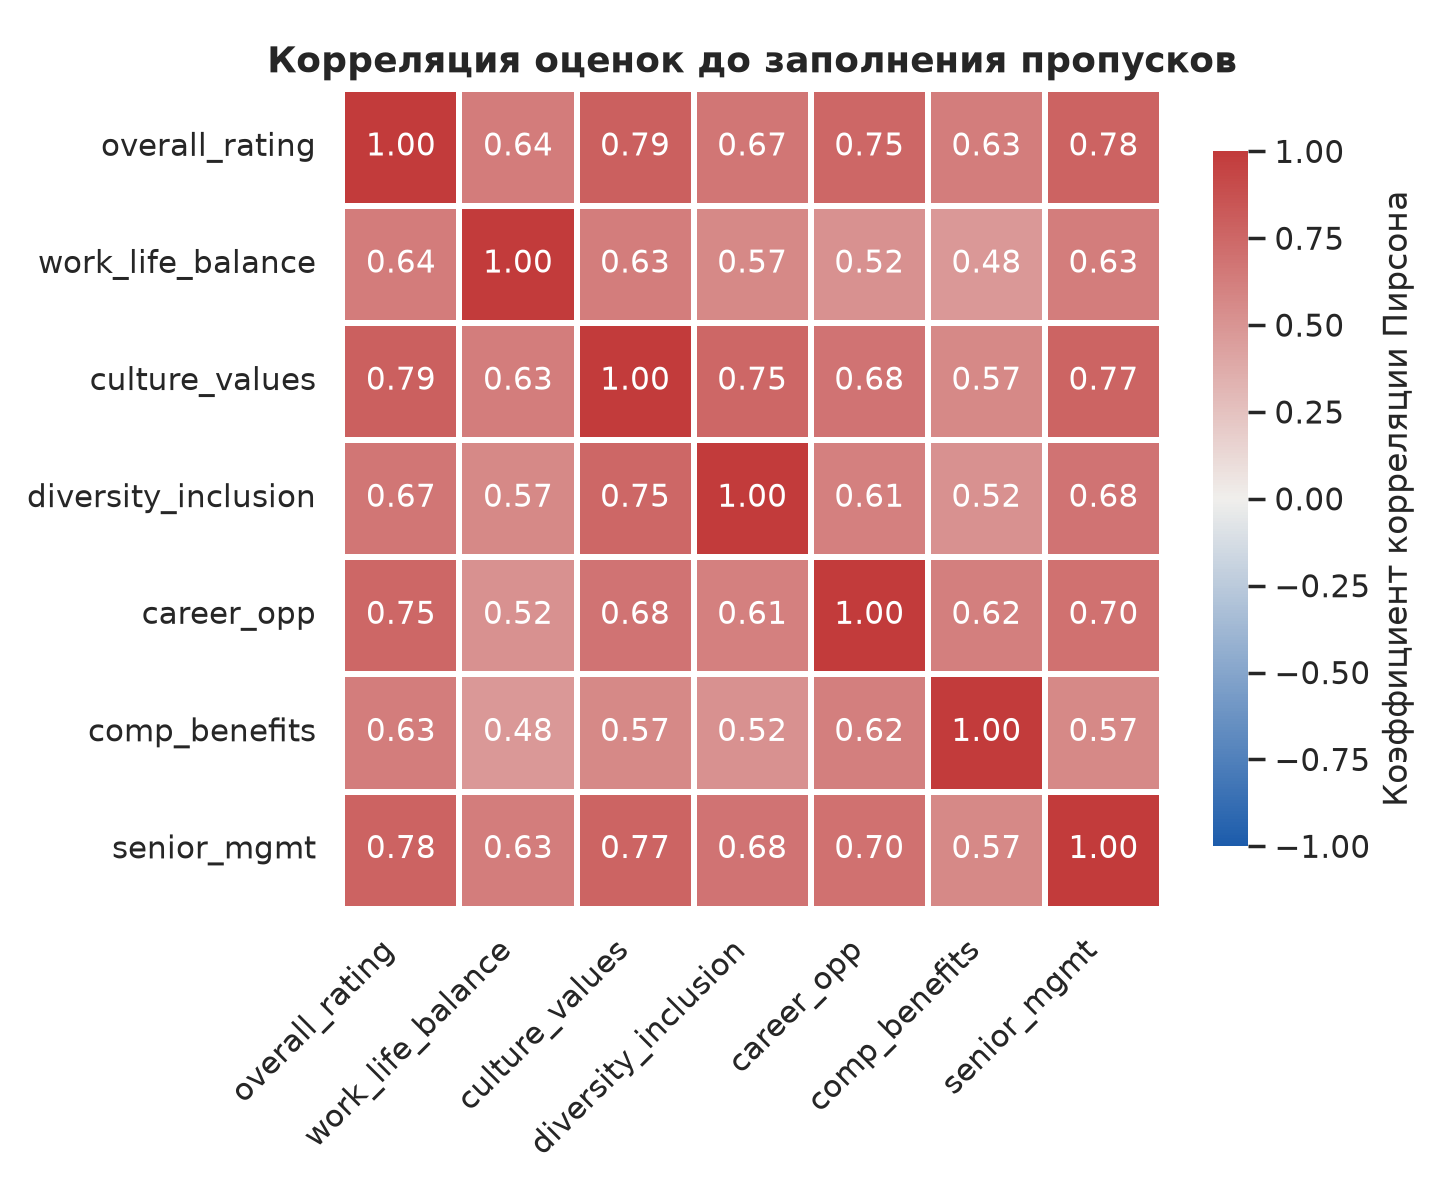
\includegraphics[width=0.7\textwidth]{Content/Images/glassdoor_corr_before.png}
    \caption{Корреляция оценок до заполнения пропусков}
    \label{fig:corr_before}
\end{figure}

Все коэффициенты положительны и лежат в диапазоне от 0,48 до 0,79, что объясняется одинаковой направленностью шкал и эффектом ореола (halo effect): довольный работодателем сотрудник склонен высоко оценивать все критерии. Сильнее всего с общей оценкой связаны культура и ценности (0,79), высшее руководство (0,78) и карьерные возможности (0,75), слабее --- разнообразие и инклюзивность (0,67), баланс работы и жизни (0,64), зарплата и льготы (0,63). Самая слабая связь (0,48) наблюдается между балансом работы и жизни и зарплатой: высокооплачиваемая работа нередко требует больше времени. Подоценка \texttt{diversity\_inclusion} тесно связана с культурой (0,75) и во многом дублирует её.

Полученный порядок совпадает с результатами исследования Glassdoor~\cite{stansell2019drivers}, в котором регрессионным анализом оценивался вклад факторов в удовлетворённость сотрудников. Наибольший вклад в нём также внесли культура и ценности (22~\%), высшее руководство (21~\%) и карьерные возможности (19~\%), а наименьший --- баланс работы и жизни (13~\%) и зарплата (12~\%). Таким образом, разведочный анализ независимо воспроизвёл вывод опубликованного исследования: удовлетворённость определяется прежде всего культурой компании и руководством, а не зарплатой.

После заполнения пропусков корреляции подоценок с общей оценкой снизились на 0,06--0,09: для культуры и ценностей --- с 0,787 до 0,700, для высшего руководства --- с 0,775 до 0,702, для баланса работы и жизни --- с 0,642 до 0,584. Причина в том, что у заполненных строк подоценка одинакова при любой общей оценке. Поэтому для оценки взаимосвязей следует опираться на коэффициенты, рассчитанные до заполнения.

Для полной корреляционной матрицы мнения закодированы как Positive~=~1, Mild~=~0, Negative~=~$-1$ (категории No opinion и Unknown в расчёте не участвуют), а статус сотрудника --- как Current~=~1, Former~=~0. Константный признак \texttt{advice\_words} в матрицу не включён, поскольку коэффициенты корреляции для него не определены. Матрица показана на рисунке~\ref{fig:corr_full}, а корреляции признаков с общей оценкой --- на рисунке~\ref{fig:corr_target}.

\begin{figure}[!ht]
    \centering
    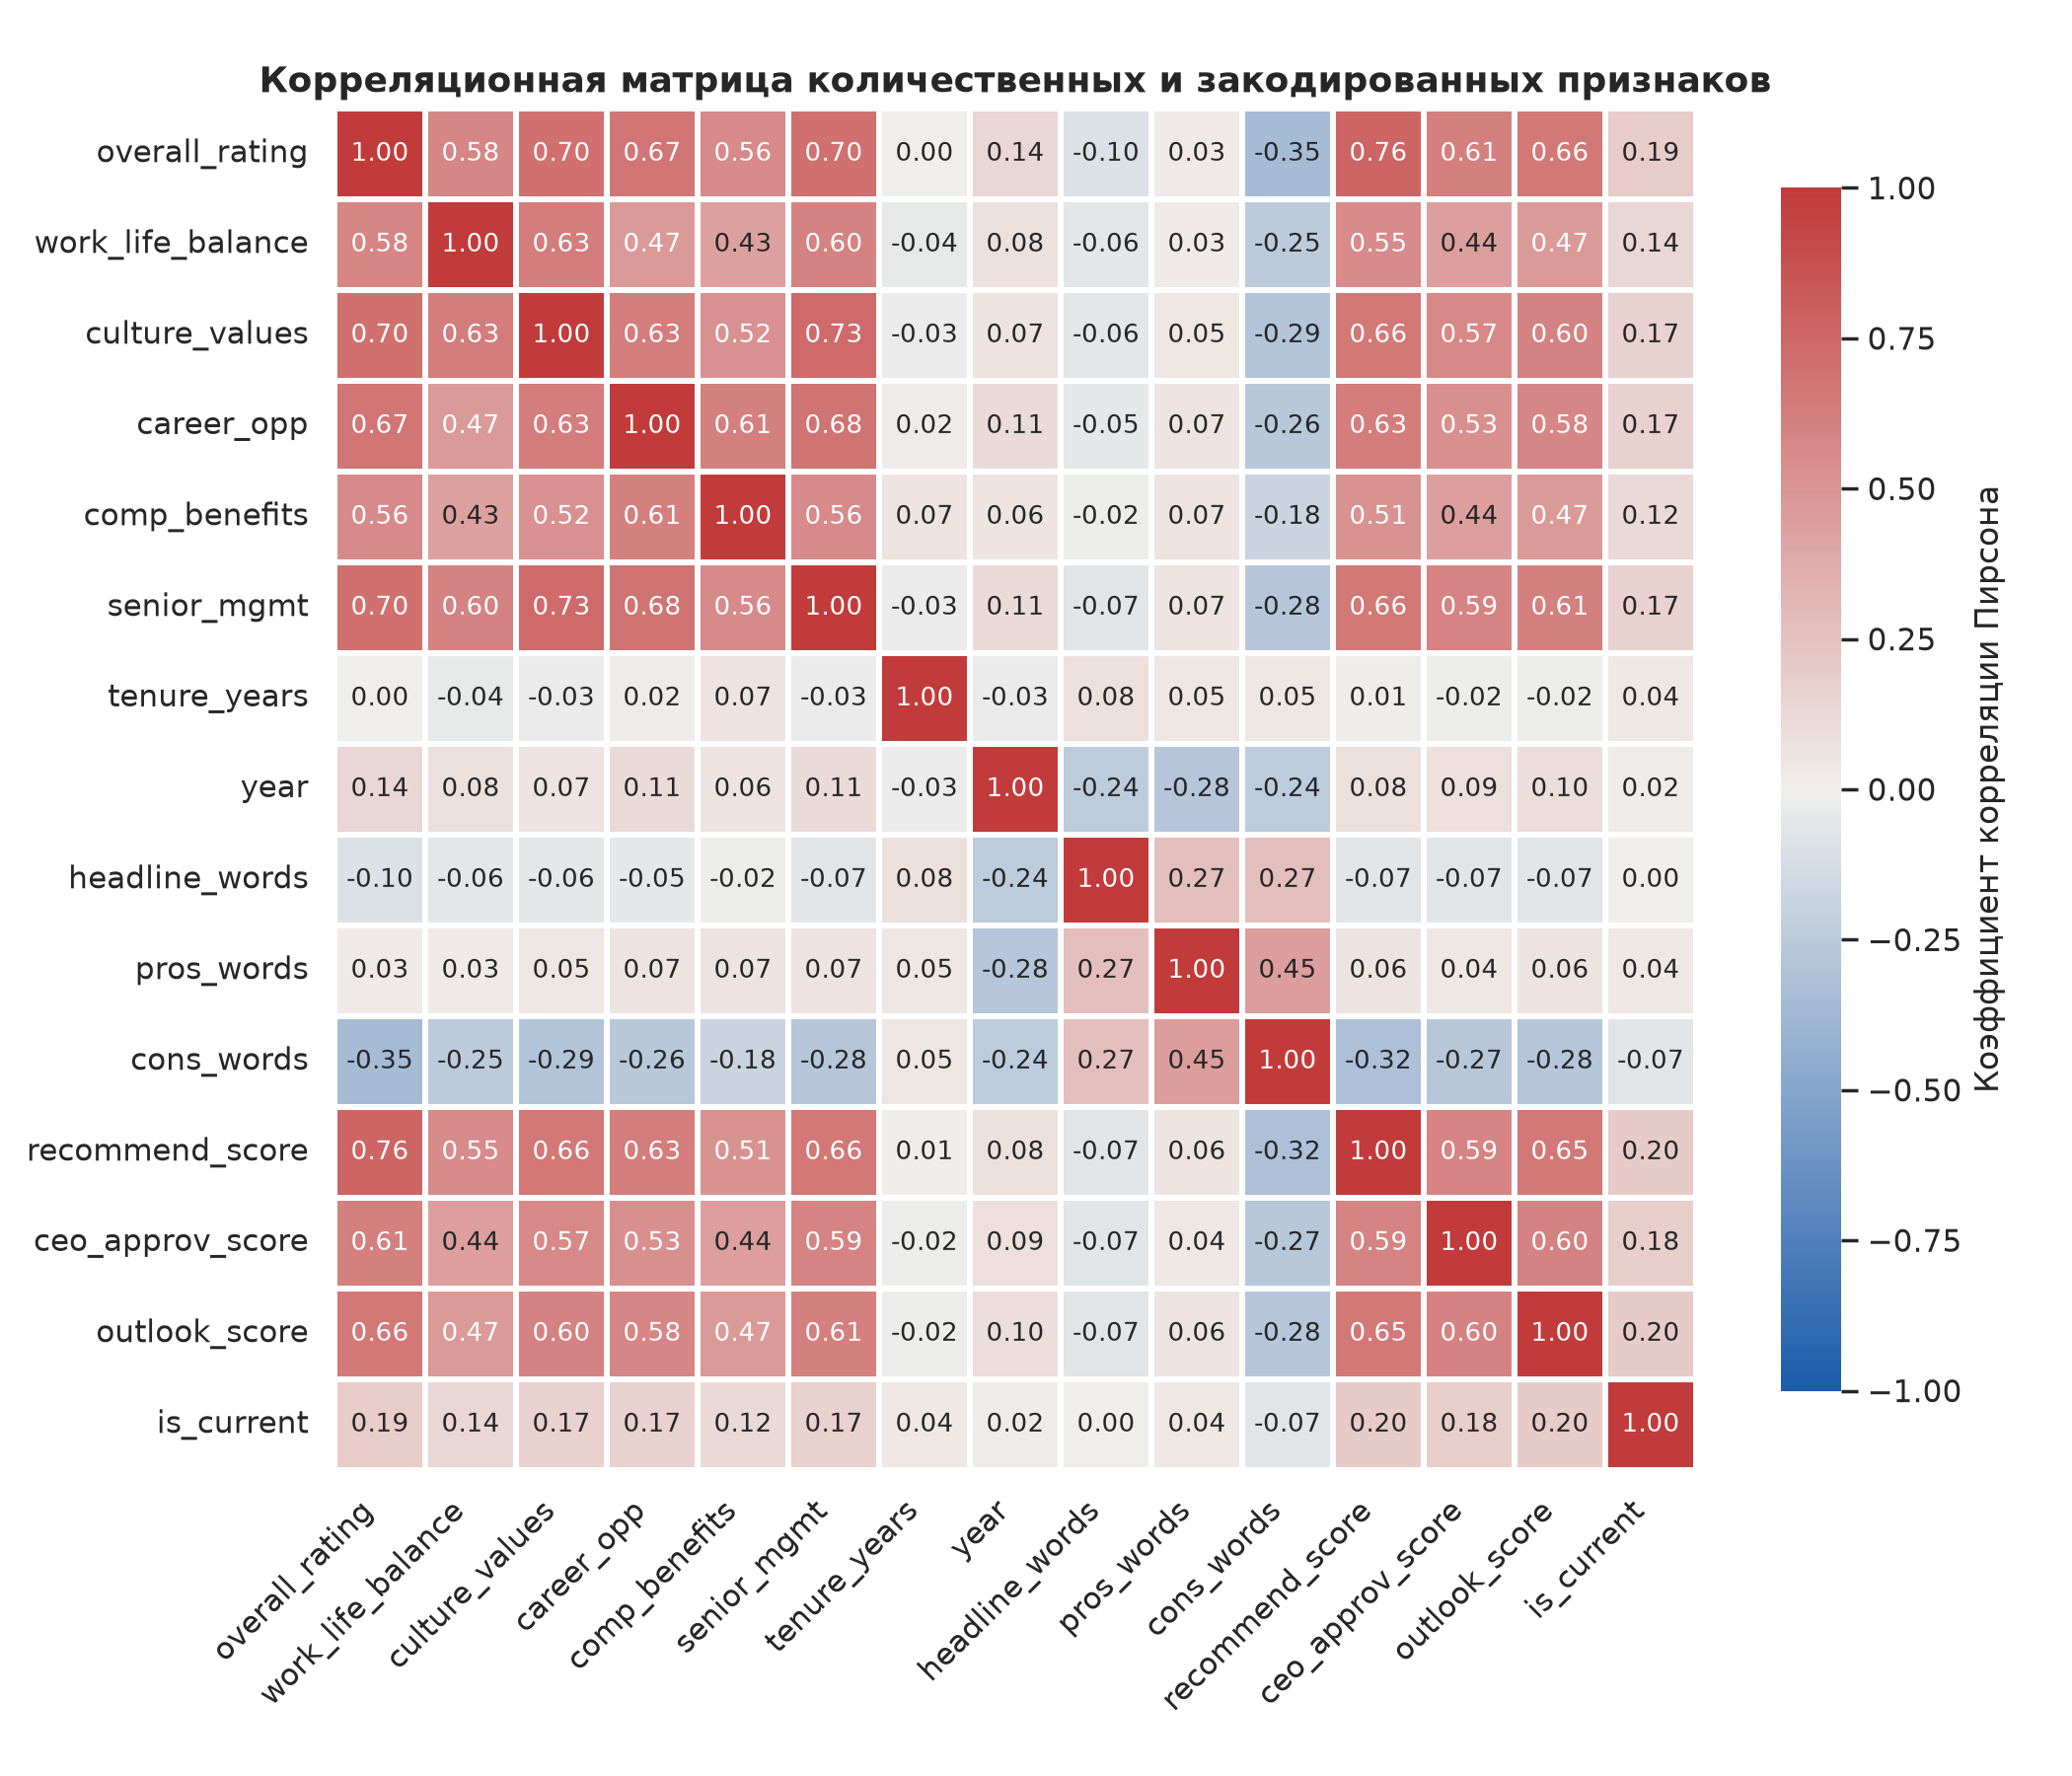
\includegraphics[width=\textwidth]{Content/Images/glassdoor_corr_full.png}
    \caption{Корреляционная матрица количественных и закодированных признаков}
    \label{fig:corr_full}
\end{figure}

\begin{figure}[!ht]
    \centering
    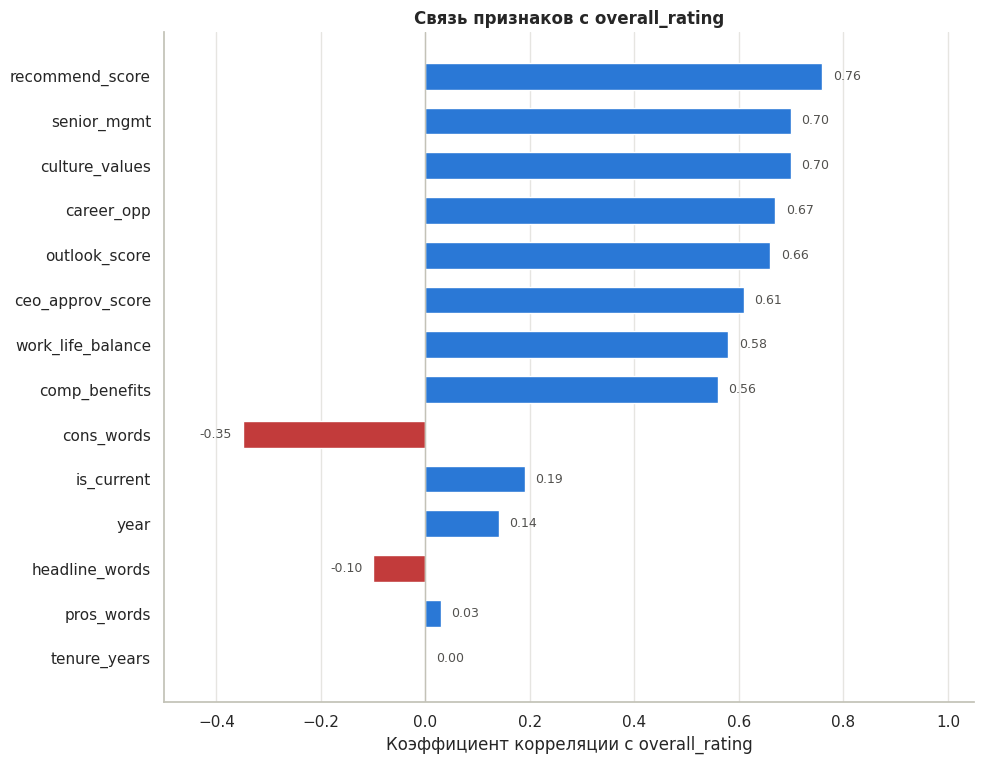
\includegraphics[width=0.62\textwidth]{Content/Images/glassdoor_target_corr.png}
    \caption{Корреляция признаков с общей оценкой}
    \label{fig:corr_target}
\end{figure}

Сильнее всего с общей оценкой связана рекомендация компании (0,76), затем подоценки руководства и культуры (по 0,70), карьерных возможностей (0,67), оценка перспектив (0,66) и одобрение генерального директора (0,61). Длина <<минусов>> отрицательно связана с общей оценкой ($-0{,}35$) и со всеми подоценками: недовольные авторы подробнее пишут о недостатках. Длина <<плюсов>> с оценкой не связана (0,03). Текущие сотрудники оценивают работодателя выше бывших (0,19). Год публикации слабо положительно связан с оценкой (0,14) и отрицательно --- с длиной текстов (от $-0{,}24$ до $-0{,}28$), то есть отзывы со временем становятся короче. Корреляция стажа с оценкой равна нулю, отчасти из-за заполнения 40~\% значений медианой, поэтому выводы о стаже следует делать по таблице~\ref{tab:tenure}.

Следует учитывать, что коэффициент Пирсона измеряет только линейную связь, а для порядковых оценок можно дополнительно рассчитать ранговый коэффициент Спирмена (класс \texttt{Correlation} пакета \texttt{pyspark.ml.stat}); корреляция также не доказывает причинно-следственной связи.

\vspace{\baselineskip}\section{Выводы}\vspace{\baselineskip}

В главе средствами Apache Spark выполнен разведочный анализ датасета Glassdoor Job Reviews~2 объёмом 3,8~ГБ, содержащего 9,9~млн отзывов о 34\,374~компаниях.

Были выявлены проблемы качества данных: 8,55~\% строк оказались полными дубликатами, почти в каждой строке был пропуск. Пропуски во многом неслучайны: совет руководству практически не заполнен, оценка разнообразия и инклюзивности отсутствует у 66~\% отзывов, стаж не указан у 40~\%. Пропуски обработаны по единым правилам, причём показано, что заполнение медианой ослабляет корреляции на 0,06--0,09. Выбросы в длине текстов устранены ограничением по 99-му перцентилю без удаления строк. Показано также, что метод IQR неприменим механически к порядковым шкалам и к распределению отзывов по компаниям, где формальные выбросы являются достоверными данными.

Средняя общая оценка составляет 3,55 и выросла с 3,05 в 2010~году до 3,72 в 2022~году. Ниже всех оценивается высшее руководство, выше всех --- корпоративная культура. Текущие сотрудники оценивают работодателя на 0,49~балла выше бывших. С общей оценкой сильнее всего связаны рекомендация компании, культура и руководство, слабее --- баланс работы и жизни и зарплата, что совпадает с выводами исследования Glassdoor.

Итоговый набор данных из 9\,055\,084~строк и 20~признаков не содержит пропусков и сохранён в таблицу \texttt{glassdoor\_reviews\_processed} формата Iceberg. Он пригоден для построения моделей машинного обучения, например для регрессии (предсказание общей оценки) и бинарной классификации (предсказание рекомендации компании).
